\subsection{КС-грамматики(продолжение)}
\begin{lemma}[о накачке]
  Пусть $L$ --- КС-язык. Тогда $\exists p \geq 1$ такое, что $\forall w \in L\colon |w| \geq p$:
  \begin{itemize}
    \item $\exists x, u, y, v, z \in \Sigma^{*}\colon w = x u y v z$
    \item $|uv| \geq 1$
    \item $|uyv| \leq p$
    \item $\forall i \geq 0\colon xu^iyv^iz \in L$
  \end{itemize}
\end{lemma}
\begin{proof} 
Пусть $L$ задаётся $(\Sigma, N, R, S)$.
Пусть $m = \max \{|\alpha| \; | \; A \to \alpha \in R\}$. Тогда $m$ --- максимально возможное число детей в дереве. Возьмем $p \coloneqq m^{|N| + 3} + 1$. 

Возьмем $|w| \geq p$. Рассмотрим минимальное по размеру дерево разбора $T$ для $w$. В $T$ есть путь $P$ длины $\geq |N| + 3$. Тогда в $P$ есть две вершины, отличающиеся от корня, с одинаковыми нетерминалами $B$.

\tikzset{every picture/.style={line width=0.75pt}} %set default line width to 0.75pt        

\center
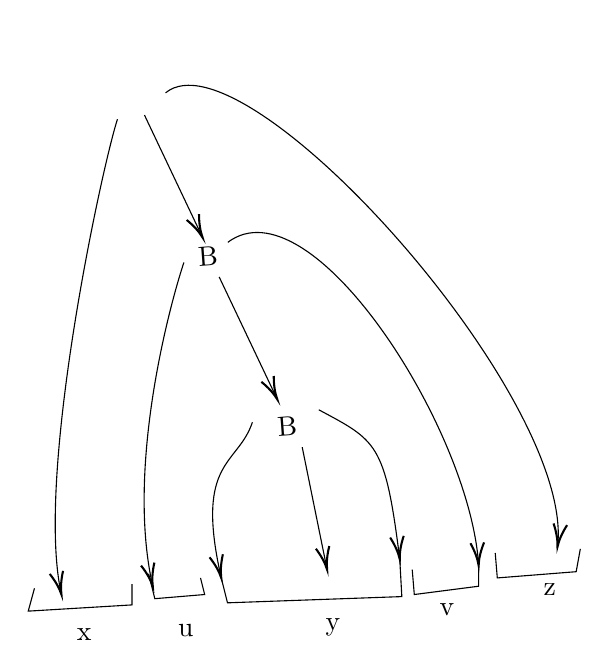
\begin{tikzpicture}[x=0.75pt,y=0.75pt,yscale=-1,xscale=1]
%uncomment if require: \path (0,300); %set diagram left start at 0, and has height of 300

%Straight Lines [id:da6656324887025324] 
\draw    (242.83,23.7) -- (269.98,80.89) ;
\draw [shift={(270.83,82.7)}, rotate = 244.61] [color={rgb, 255:red, 0; green, 0; blue, 0 }  ][line width=0.75]    (10.93,-3.29) .. controls (6.95,-1.4) and (3.31,-0.3) .. (0,0) .. controls (3.31,0.3) and (6.95,1.4) .. (10.93,3.29)   ;
%Straight Lines [id:da2587378767927274] 
\draw    (278.83,101.7) -- (305.98,158.89) ;
\draw [shift={(306.83,160.7)}, rotate = 244.61] [color={rgb, 255:red, 0; green, 0; blue, 0 }  ][line width=0.75]    (10.93,-3.29) .. controls (6.95,-1.4) and (3.31,-0.3) .. (0,0) .. controls (3.31,0.3) and (6.95,1.4) .. (10.93,3.29)   ;
%Straight Lines [id:da20646266691180049] 
\draw    (318.83,183.7) -- (330.43,240.74) ;
\draw [shift={(330.83,242.7)}, rotate = 258.5] [color={rgb, 255:red, 0; green, 0; blue, 0 }  ][line width=0.75]    (10.93,-3.29) .. controls (6.95,-1.4) and (3.31,-0.3) .. (0,0) .. controls (3.31,0.3) and (6.95,1.4) .. (10.93,3.29)   ;
%Curve Lines [id:da7872440698430629] 
\draw    (326.83,165.7) .. controls (354.55,180.55) and (358.75,181.68) .. (365.62,236.04) ;
\draw [shift={(365.83,237.7)}, rotate = 262.87] [color={rgb, 255:red, 0; green, 0; blue, 0 }  ][line width=0.75]    (10.93,-3.29) .. controls (6.95,-1.4) and (3.31,-0.3) .. (0,0) .. controls (3.31,0.3) and (6.95,1.4) .. (10.93,3.29)   ;
%Curve Lines [id:da4699624977272372] 
\draw    (283,85) .. controls (322.8,55.15) and (399.07,173.51) .. (403.77,239.71) ;
\draw [shift={(403.83,240.7)}, rotate = 266.53] [color={rgb, 255:red, 0; green, 0; blue, 0 }  ][line width=0.75]    (10.93,-3.29) .. controls (6.95,-1.4) and (3.31,-0.3) .. (0,0) .. controls (3.31,0.3) and (6.95,1.4) .. (10.93,3.29)   ;
%Curve Lines [id:da43611075880270866] 
\draw    (253,13) .. controls (290.64,-18.14) and (449.24,157.93) .. (441.96,230.61) ;
\draw [shift={(441.83,231.7)}, rotate = 277.13] [color={rgb, 255:red, 0; green, 0; blue, 0 }  ][line width=0.75]    (10.93,-3.29) .. controls (6.95,-1.4) and (3.31,-0.3) .. (0,0) .. controls (3.31,0.3) and (6.95,1.4) .. (10.93,3.29)   ;
%Curve Lines [id:da2099655325914782] 
\draw    (294.83,171.7) .. controls (287.9,192.49) and (267.25,189.76) .. (279.45,245.01) ;
\draw [shift={(279.83,246.7)}, rotate = 257.15] [color={rgb, 255:red, 0; green, 0; blue, 0 }  ][line width=0.75]    (10.93,-3.29) .. controls (6.95,-1.4) and (3.31,-0.3) .. (0,0) .. controls (3.31,0.3) and (6.95,1.4) .. (10.93,3.29)   ;
%Curve Lines [id:da4027421379797006] 
\draw    (261.83,94.7) .. controls (254.9,115.49) and (234.25,192.15) .. (246.45,248.98) ;
\draw [shift={(246.83,250.7)}, rotate = 257.15] [color={rgb, 255:red, 0; green, 0; blue, 0 }  ][line width=0.75]    (10.93,-3.29) .. controls (6.95,-1.4) and (3.31,-0.3) .. (0,0) .. controls (3.31,0.3) and (6.95,1.4) .. (10.93,3.29)   ;
%Curve Lines [id:da41729749785096726] 
\draw    (229.83,25.7) .. controls (222.9,46.49) and (190.49,194.69) .. (202.46,252.96) ;
\draw [shift={(202.83,254.7)}, rotate = 257.15] [color={rgb, 255:red, 0; green, 0; blue, 0 }  ][line width=0.75]    (10.93,-3.29) .. controls (6.95,-1.4) and (3.31,-0.3) .. (0,0) .. controls (3.31,0.3) and (6.95,1.4) .. (10.93,3.29)   ;
%Shape: Polygon [id:ds7926596968899329] 
\draw   (236.83,249.7) -- (236.83,259.7) -- (186.83,262.7) -- (186.83,262.7) -- (189.83,251.7) -- (186.83,262.7) -- (236.83,259.7) -- cycle ;
%Shape: Polygon [id:ds9488989205346039] 
\draw   (269.83,246.7) -- (271.83,254.7) -- (247.83,256.7) -- (247.83,256.7) -- (244.83,244.7) -- (247.83,256.7) -- (271.83,254.7) -- cycle ;
%Shape: Polygon [id:ds12424328286302411] 
\draw   (365.83,237.7) -- (366.83,255.7) -- (282.83,258.7) -- (282.83,258.7) -- (279.83,246.7) -- (282.83,258.7) -- (366.83,255.7) -- cycle ;
%Shape: Polygon [id:ds18937668092041682] 
\draw   (452.83,232.7) -- (450.83,243.7) -- (412.83,246.7) -- (412.83,246.7) -- (411.83,234.7) -- (412.83,246.7) -- (450.83,243.7) -- cycle ;
%Shape: Polygon [id:ds4743806575119506] 
\draw   (403.83,240.7) -- (403.83,250.7) -- (372.83,254.7) -- (372.83,254.7) -- (371.83,242.7) -- (372.83,254.7) -- (403.83,250.7) -- cycle ;

% Text Node
\draw (305.22,168.17) node [anchor=north west][inner sep=0.75pt]  [rotate=-355.72] [align=left] {B};
% Text Node
\draw (267.05,86.54) node [anchor=north west][inner sep=0.75pt]  [rotate=-355.72] [align=left] {B};
% Text Node
\draw (209,270) node [anchor=north west][inner sep=0.75pt]   [align=left] {x};
% Text Node
\draw (257.83,267.7) node [anchor=north west][inner sep=0.75pt]   [align=left] {u};
% Text Node
\draw (328.83,265) node [anchor=north west][inner sep=0.75pt]   [align=left] {y};
% Text Node
\draw (433.83,248.2) node [anchor=north west][inner sep=0.75pt]   [align=left] {z};
% Text Node
\draw (383.83,258) node [anchor=north west][inner sep=0.75pt]   [align=left] {v};
\end{tikzpicture}

Присвоим $x, u, y, v, z$ как выставлено на рисунке. 
\begin{itemize}
  \item Ситуация $|u| = |v| = 0$ произойти не может, так как тогда после первой $B$ мы просто прошлись по циклу до второй, а значит мы можем переместить нижнее поддерево на место первой $B$-ки и только уменьшить наше поддерево, противоречие. Таким образом доказали, что $|uv| \geqslant 1$.
  \item Если случилось, что $|uyv| > p$, то давайте решим задачу для поддерева первой $B$-ки (мы взяли её так, что она не равна корню), и просто добавим $x$ к $x_B$ слева и $z$ к $z_B$ справа.
  \item Почему верно последнее свойство? Потому что вместо того чтобы пойти на второй $B$-ке в поддерево, образующее $y$ мы могли бы просто повторить то что сделали раннее --- разветвится на $u$ и на $v$ и после этого опять дойти до $B$. Таким образом мы можем спавнить бесконечное количество $u$-шек и $v$-шек по бокам от $y$ (в том числе 0).
\end{itemize}
\end{proof}

\textbf{Пример.} Язык $L = \{ a^n b^n c^n \mid n \geqslant 0 \}$ не задаётся КС-грамматикой. 
\begin{proof}
  От противного. Пусть задаётся $(\Sigma, N, R, S)$. Тогда возьмём $p$ из леммы о накачке и $w = a^p b^p c^p$. Действительно, $\abs{w} \geqslant p$. Значит, найдутся $x, u, y, v, z \in \Sigma^{*}$, т.ч. $w = x u y v z$, которые удовл. условиям леммы. Разберём случаи:
  \begin{itemize}
    \item $u$ или $v$ содержит разные символы. Знаем, что $x u^i y v^i z$. Тогда при $i$ хотя бы 2, будет уже слишком много чередования символов. Таким образом, каждый из $u$ и $v$ не содержит разных символов.
    \item $u, v \in a^*$. Тогда применим лемму к $i=0$. $xyz \in L$, но в $xyz$ меньше символов $a$, чем в $w=xuyvz$, а $b$ и $c$ такое же количество.
    \item $u \in a^*$, $v \in b^*$. Тогда опять же $xyz \in L$, но в нём меньше символов $a$ и $b$, чем в $w$, а символов $c$ столько же.
    \item Аналогично для остальных комбинаций.
  \end{itemize}
\end{proof}

На основе предыдущего примера можно показать, что КС-грамматик не хватает для проверки программ на языках программирования. При этом их хватает для разбора арифметических выражений.

\textbf{Пример.} Рассмотрим программу на языке C:
\begin{lstlisting}[language=C]
  int main(void) = { int x...x; x...x = x...x; }
\end{lstlisting}
Пусть первый идентификатор состоит из $i$ символов $x$, второй --- из $j$, третий --- из $k$. Тогда программа корректна тогда и только тогда, когда $i = j = k$. Иначе переменная не определена. Ну аналогично предыдущему примеру по лемме о накачке можно доказать, что такое КС-грамматикой не распознаётся.

\textbf{Замечание конспектирующего.} На мой взгляд, это совершенно беспонтовый пример, потому что не понятно, зачем нужно пытаться сразу и синтаксис, и семантику проверять одним проходом. Ошибка неопределённого идентификатора к синтаксису никак не относится и после разбора синтаксиса тривиально проверяется.

\begin{theorem}
  Множество КС-языков не замкнуто относительно пересечения и дополнения.
\end{theorem}
\begin{proof} \quad
  \begin{itemize}
    \item \textbf{Пересечение}. Пусть $L_1 = \{a^i b^l c^l \; | \; i, l \geq 0\}$, $L_2  = \{a^m b^m c^j \; | \; m, j \geq 0\}$. 

    Выше уже поняли, что $L_1 \cap L_2 = \{a^n b^n c^n \; | \; n \geq 0\}$ --- не КС. Осталось показать, что и $L_1$ и $L_2$ --- КС-языки. Действительно, посмотрим на следующие грамматики. Для языка $L_1$:
     \begin{align*}
       S_1 &\to aS_1 \; | \; A \\
       A &\to bAc \; | \; \varepsilon
     \end{align*}
     Для языка $L_2$:
     \begin{align*}
       S_2 &\to S_1c \; | \; B \\
       B &\to aBb \; | \; \varepsilon
     \end{align*}
     Легко видеть, что обе грамматики делают то что нужно.
    \item \textbf{Дополнение}. Пусть это не так, тогда заметим, что
    \begin{equation*}
      L_1 \cap L_2 = \overline{\overline{L_1} \cup \overline{L_2}}
    \end{equation*}
    где $\overline{A}$ в данном случае это $(L_1 \cup L_2) \backslash A$. Но тогда $L_1 \cap L_2$ всегда контекстно-свободен, а это не так.
  \end{itemize}
\end{proof}

\begin{conj}
  Унарный язык --- это подмножество $\{0\}^{*}$.
\end{conj}
\begin{theorem}
  Регулярный унарный язык --- это объединение конечного числа арифметических прогрессий $\{0^{ak + b} \; | \; k \geq 0\}$ и конечного множества.
\end{theorem}
\begin{proof}
  Действительно, по лемме о накачке такие и только такие языки являются регулярными.
\end{proof}
\begin{theorem}
  Унарный КС язык --- это объединение конечного числа арифметических прогрессий $\{0^{ak + b} \; | \; k \geq 0\}$ и конечного множества.
\end{theorem}
\begin{proof}
  Действительно, здесь тоже работает лемма о накачке.
\end{proof}
\begin{follow}
  Унарные регулярные языки и унарные КС языки --- это одно и то же.
\end{follow}

\subsection{Нормальная форма для КС грамматик Хомского}
  Оказывается, у грамматик бывает нормальная форма.
  
\begin{conj}
  Итак, КС-грамматика находится в \sout{головной нормальной форме} \textbf{нормальной форме Хомского}, если любое правило имеет один из следующих видов:
  \begin{itemize}
    \item $S \to \varepsilon$, т.е. из \textbf{начального} нетерминала мы можем выводить пустую строку;
    \item $S$ не используется в правых частях правил;
    \item $A \to BC$, где $B, C$ --- нетерминалы;
    \item $A \to a$, где $a \in \Sigma$.
  \end{itemize}
\end{conj}

\begin{theorem}
  Для любой КС-грамматики можно построить эквивалентную КС-грамматику в нормальной форме Хомского, т.е. которая задает тот же язык.
\end{theorem}
\begin{proof} \quad

  \begin{enumerate}
    \item Сокращение правых частей. Рассмотрим правило следующего вида: $A \to \alpha$, где $|\alpha| \geq 3$. Вместо этого правила добавим $|\alpha|$ новых правил:
    \begin{align*}
      &A \to \alpha_1 A' \\
      &A' \to \alpha_2 A'' \\
      & \vdots \\
      &A^{(|\alpha| - 1)} \to \alpha_{|\alpha|}
    \end{align*}
    где нетерминалы $A', A'', \dotsc, A^{(|\alpha| - 1)}$ свои для каждой строки $\alpha$. Таким образом длины всех правых частей теперь не превосходят двух.
    
    Рассмотрим какие типы правил у нас остались:
    \begin{itemize}
      \item $A \to \varepsilon$
      \item $A \to a$
      \item $A \to B$
      \item $A \to ab, A \to aB, A \to Ba, A \to CD$
    \end{itemize}
    Заметим, что для исправления проблемы в последнем типе правил мы можем создать по нетерминальному символу $N_c$ для каждого символа $c$, добавить правила $N_c \to c$ и просто заменить правила соответствующим образом:
    \begin{align*}
      A \to ab &\implies A \to N_a N_b \\
      A \to aB &\implies A \to N_a B \\
      A \to Ba &\implies A \to B N_a
    \end{align*}

    \item Избавимся от $S$ в правых частях. Давайте просто создадим еще один нетерминал $S'$, скопируем для него все правила, которые были верны для $S$, а также во всем списке правил во всех правых частях заменим $S$ на $S'$.
    
    \item Избавимся от правил $A \to \varepsilon$ в случае $A \neq S$. Построим множество $\mathrm{NULL}$, которое будет состоять из всех нетерминалов из которых выводится пустая строка. Будем строить его по шагам: на очередном шаге алгоритма пробегаемся по всем нетерминалам не из $\mathrm{NULL}$ и проверяем следующее:

    Если для текущего нетерминала $A$ существует правило $A \to \varepsilon$ или правило $A \to \alpha$ где $\alpha$ такое, что $\forall i\colon \alpha_i \in \mathrm{NULL}$. Тогда добавляем нетерминал $A$ в $\mathrm{NULL}$. Легко видеть, что все элементы множества $\mathrm{NULL}$ и только они могут быть найдены таким таким способом. 
    Останавливать алгоритм будем на моменте, когда на очередном шаге не нашли ни одного нового элемента $\mathrm{NULL}$.

    Теперь используем эту информацию чтобы преобразовать наши правила. Во-первых удалим все правила вида $A \to \varepsilon$, где $A \neq S$. Во-вторых для всех правил $A \to BC$, где $B \in \mathrm{NULL}$ добавим правило $A \to C$, а если $C \in \mathrm{NULL}$, то добавим правило $A \to B$.

    \textbf{Утверждение.} После такого преобразования все, что выводится из нетерминального символа --- это то, что было раньше, за исключением пустой строки.

    \item Избавимся от правил вида $A \to B$, где $B \in N$. Для каждой пары $A, \alpha$ такой, что $A \in N$ и $\alpha \in \Sigma \cup \{CD \; | \; C, D \in N\}$ добавим правило $A \to \alpha$ если существует такая $A_1, \dotsc, A_k$ такая, что:
    \begin{equation*}
      A \to A_1, A_1 \to A_2, \dotsc, A_k \to \alpha
    \end{equation*}
    После этого все правила $A \to B$ удалим.

    Альтернативное решение (простой, но непроверенный кукарек): 
    Заменим все правила $B \to \gamma$ на $A \to \gamma$ и избавимся от правила $A \to B$ (чем-то похоже на транзитивное замыкание). Будем повторять такие действия, пока правил такого вида не останется. Только начиная с какого-то шага у нас могли получиться правила $A \to A$, если у нас правило $A \to B$ лежало на цикле. От таких правил можно безопасно избавиться --- они бесполезны.
  \end{enumerate}
\end{proof}
\subsection{Синтаксический анализ}
Дана грамматика $(\Sigma, N, R, S)$. Нужно:
\begin{enumerate}
  \item Построить разрешающий алгоритм для языка, который задается этой грамматикой.
  \item Построить дерево разбора.
\end{enumerate}
Алгоритм будет следующим:
\begin{enumerate}
  \item Привести грамматику в нормальную форму Хомского.
  \item Решаем задачу методом динамического программирования. Пусть $x = x_1\dotso x_n$ --- строка, которую мы анализируем. Тогда будем считать следующую функцию: $T_{i, j}$ для $i \leq j \in [n]$ --- это множество нетерминальных символов, из которых выводится $x_i \dotsc x_j$. Тогда 
    \begin{equation*}
      S \in T_{1, n} \iff x \in L
    \end{equation*}
  \begin{itemize}
    \item База. $T_{i, i}$ это все такие $A \in N$, для которых существует правило $A \to x_i$.
    \item Переход. $T_{i, j}$ это все такие $A$, для которых $\exists B,C \in N, k \in [i, j)$ такие, что $A \to BC, B \in T_{i, k}, C \in T_{k + 1, j}$.
  \end{itemize}
  Если считать грамматику константой, то легко видеть что время работы такого алгоритма есть $\mathcal{O}(n^3)$.
  \item Строим дерево разбора в терминах грамматики в нормальной форме. Будем реализовывать такой алгоритм $\mathrm{create\_tree(A, k, s)}$: дан нетерминал $A$, даны индексы $k, s$. Тогда нам нужно построить дерево разбора для строки $x_k, \dotsc, x_s$, в корне которого находится $A$. 

  Тогда если $k = s$, то просто ищем правило перехода из $A$ в $x_k$. И из корня ведем ребро в лист с символом $x_k$. Иначе мы должны преобразовать текущий нетерминал в два нетерминала, а значит ищем такое правило $A \to BC$, где $\exists j\colon B \in T_{k, j}, C \in T_{j + 1, s}$. Тогда из корня проводим два ребра в сыновей с символами $B$ и $C$ и запускаем рекурсивно алгоритм от $\mathrm{create\_tree(B, k, j)}$ и $\mathrm{create\_tree(C, j + 1, s)}$.

  Оценим время работы алгоритма. Заметим, что каждое ветвление(второй случай в алгоритме) мы проводим <<черту>> в строке после символа с индексом $j$, означающую, что теперь символы до $j$-го и после будут находится в разных поддеревьях. Но всего черт можно провести $n - 1$ штуку --- между каждой парой соседних символов. То есть в дереве максимум $n - 1$ вершина с ветвлением. При этом в дереве ровно $n$ листов. Таким образом в дереве максимум $2n - 1$ вершин(и даже, кажется, ровно столько). При этом каждая итерация алгоритма в конкретной вершине работает за $\mathcal{O}(n)$. Таким образом время работы алгоритма $\mathcal{O}(n^2)$.
\end{enumerate}
